\documentclass[12pt]{article}
% Geometria i fonty jak w szablonie prowadzacego: letterpaper, 12pt, bez geometry.
\usepackage{iftex}
\ifPDFTeX
  \usepackage[utf8]{inputenc}
\else
  \usepackage{fontspec}
  \setmainfont{lmroman10-regular.otf}[
    BoldFont       = lmroman10-bold.otf,
    ItalicFont     = lmroman10-italic.otf,
    BoldItalicFont = lmroman10-bolditalic.otf]
\fi
\usepackage[polish]{babel}
\usepackage{amsmath,amssymb}
\usepackage{booktabs}
\usepackage{graphicx}
\usepackage{caption}
\addto\captionspolish{\renewcommand{\refname}{Bibliografia}}

\title{\textbf{Zadanie nr 3 - perceptron wielowarstwowy 4-2-4}\\[2mm]
       \large Inteligentna Analiza Danych}
\author{Łukasz Centkowski 264303 \\ Maciej Dominiak 264307}
\date{25 października 2026}

\begin{document}
\maketitle
\thispagestyle{empty}
\newpage

\section{Cel zadania}

Zadanie polegało na wytrenowaniu perceptronu wielowarstwowego o~architekturze
4-2-4 tak, aby kopiował swoje wejścia na wyjścia. Sprawdziliśmy przy tym, czy
trening jest w~ogóle możliwy, gdy neurony warstwy wyjściowej nie mają wejść
obciążających, oraz dlaczego tak się dzieje.

\section{Wstęp teoretyczny}

Sieć ma trzy warstwy: cztery neurony kopiujące na wejściu, dwa liniowe bez biasu
w~warstwie ukrytej i~cztery sigmoidalne z~biasem na wyjściu. Razem 20 parametrów,
czyli 16 wag i~4 biasy. Trening to wsteczna propagacja błędu~\cite{rumelhart},
czyli gradientowa minimalizacja funkcji
\begin{equation}
E(\mathbf{w}) \;=\; \tfrac{1}{2}\sum_{\mu}\sum_{i}
\bigl(z_i^{(\mu)} - y_i^{(\mu)}\bigr)^2 .
\label{eq:blad}
\end{equation}
Zatrzymuje ją wyłącznie zadana liczba epok $L$, bez progu
błędu~\cite{wyklad,osowski}.

Kluczowe jest to, co robi pojedynczy neuron wyjściowy. Dostaje z~warstwy ukrytej
dwie liczby, czyli \emph{punkt na płaszczyźnie}, i~ma dać wartość bliską~1 dla
swojego wzorca, a~bliską~0 dla trzech pozostałych. Jego granica decyzyjna to
prosta
\begin{equation}
\mathbf{u}\cdot\mathbf{h} + b = 0 ,
\label{eq:granica}
\end{equation}
gdzie $\mathbf{u}$ to wagi, a~$b$ bias. Bez biasu zostaje
$\mathbf{u}\cdot\mathbf{h} = 0$, a~taka prosta \textbf{zawsze przechodzi przez
punkt $(0,0)$}.

\section{Eksperymenty i wyniki}

Zbiór treningowy to cztery wzorce autoasocjacji: $\mathbf{x} = \mathbf{z} =
[1,0,0,0]$, $[0,1,0,0]$, $[0,0,1,0]$ oraz $[0,0,0,1]$. We wszystkich
eksperymentach użyliśmy kroku uczącego $0{,}5$ i~20000 epok, a~każdy wariant
powtórzyliśmy 10 razy od różnych wag losowych z~przedziału $[-1,1]$.

\subsection{Eksperyment nr 1: trening z~wejściami obciążającymi}

\subsubsection{Założenia}
Architektura dokładnie taka, jak w~treści zadania: neurony wyjściowe mają
wejścia obciążające.

\subsubsection{Przebieg}
Dziesięć przebiegów od różnych wag startowych. Po każdej epoce notowaliśmy
wartość funkcji~(\ref{eq:blad}).

\subsubsection{Rezultat}
Błąd końcowy wyniósł od $0{,}000116$ do $0{,}000122$, czyli we wszystkich
przebiegach praktycznie tyle samo. Wyjścia najlepszego przebiegu zawiera
Tab.~\ref{tab:zbias}.

\begin{table}[h]
\centering
\caption{Wyjścia sieci z~wejściami obciążającymi}
\label{tab:zbias}
\begin{tabular}{ccccc}
\toprule
\textbf{Wzorzec} & $y_1$ & $y_2$ & $y_3$ & $y_4$ \\
\midrule
1 & \textbf{0,998} & 0,005 & 0,000 & 0,007 \\
2 & 0,005 & \textbf{0,998} & 0,007 & 0,000 \\
3 & 0,000 & 0,003 & \textbf{0,997} & 0,005 \\
4 & 0,003 & 0,000 & 0,004 & \textbf{0,996} \\
\bottomrule
\end{tabular}
\end{table}

Sieć odtwarza wszystkie cztery wzorce. Właściwe wyjście ma wartość bliską
jedności, a~pozostałe trzy są wygaszone poniżej $0{,}01$.

\subsection{Eksperyment nr 2: trening bez wejść obciążających}

\subsubsection{Założenia}
Ta sama architektura i~te same parametry, ale neurony wyjściowe pozbawione
biasów. Liczba parametrów spada z~20 do~16.

\subsubsection{Przebieg}
Jak w~eksperymencie nr~1. Dodatkowo sprawdziliśmy, czy wynik nie bierze się
z~niedouczenia, powtarzając trening dla trzech kroków uczących i~dwóch długości
treningu.

\subsubsection{Rezultat}
Błąd końcowy wyniósł od $0{,}384495$ do $0{,}444623$, a~więc ponad 3300 razy
więcej niż z~biasami. Wyjścia najlepszego przebiegu zawiera
Tab.~\ref{tab:bezbias}.

\begin{table}[h]
\centering
\caption{Wyjścia sieci bez wejść obciążających}
\label{tab:bezbias}
\begin{tabular}{cccccl}
\toprule
\textbf{Wzorzec} & $y_1$ & $y_2$ & $y_3$ & $y_4$ & \\
\midrule
1 & \textbf{1,000} & 0,166 & 0,154 & 0,582 & źle, fałszywe $y_4$ \\
2 & 0,000 & \textbf{1,000} & 0,018 & 0,016 & dobrze \\
3 & 0,019 & 0,151 & \textbf{1,000} & 0,000 & dobrze \\
4 & 0,052 & 0,570 & 0,000 & \textbf{0,834} & źle, fałszywe $y_2$ \\
\bottomrule
\end{tabular}
\end{table}

Dwa wzorce sieć odtwarza czysto, a~przy dwóch pozostałych zapala wprawdzie
właściwe wyjście, ale \emph{nie potrafi wygasić fałszywego}: $y_4 = 0{,}582$
przy wzorcu~1 i~$y_2 = 0{,}570$ przy wzorcu~4, choć oba powinny wynosić zero.
Stąd bierze się cały błąd resztkowy.

Wynik nie jest skutkiem zbyt krótkiego treningu, co pokazuje
Tab.~\ref{tab:krok}.

\begin{table}[h]
\centering
\caption{Najlepszy błąd bez biasów przy różnych parametrach treningu}
\label{tab:krok}
\begin{tabular}{ccc}
\toprule
\textbf{Krok uczący} & \textbf{Epoki} & \textbf{Najlepszy błąd} \\
\midrule
0,1 & 20000 & 0,420717 \\
0,1 & 50000 & 0,381481 \\
0,5 & 20000 & 0,384495 \\
0,5 & 50000 & 0,396724 \\
2,0 & 20000 & 0,634560 \\
2,0 & 50000 & 0,631445 \\
\bottomrule
\end{tabular}
\end{table}

Ani wydłużenie treningu, ani zmiana kroku uczącego nie zbijają błędu poniżej
około $0{,}38$. To jest faktyczna granica, a~nie niedouczenie. Porównanie
przebiegu zbieżności obu wariantów przedstawia Rys.~\ref{fig:zbieznosc}.

\begin{figure}[htbp]
\centering
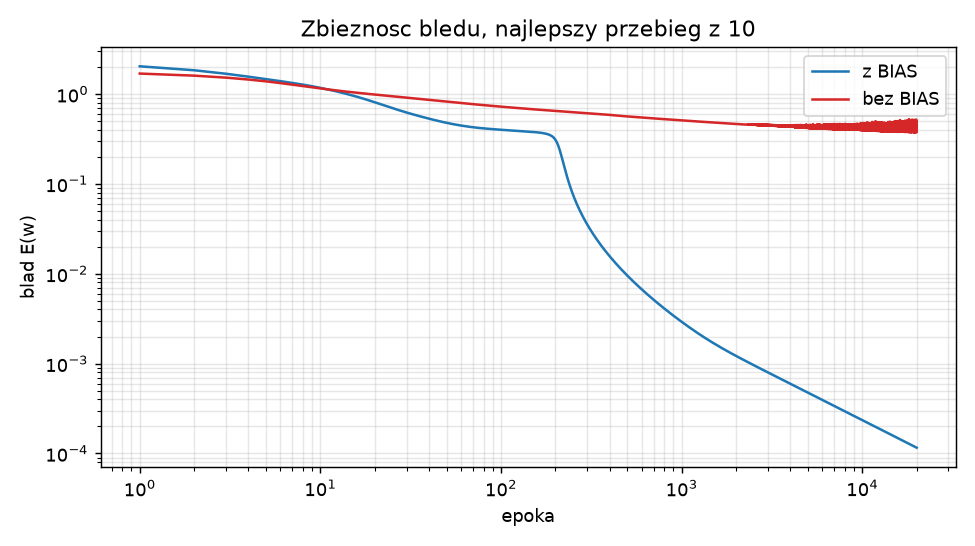
\includegraphics[width=\textwidth]{wyniki/zbieznosc.png}
\caption{Zbieżność błędu w~najlepszym z~dziesięciu przebiegów}
\label{fig:zbieznosc}
\end{figure}

\subsection{Eksperyment nr 3: geometria warstwy ukrytej}

\subsubsection{Założenia}
Warstwa ukryta ma dwa neurony, więc każdy wzorzec staje się punktem na
płaszczyźnie. Chcieliśmy sprawdzić, ile z~czterech punktów da się oddzielić
prostą od pozostałych trzech, osobno dla prostej dowolnej i~dla prostej
przechodzącej przez początek układu.

\subsubsection{Przebieg}
Dla najlepszego przebiegu każdego wariantu odczytaliśmy położenia czterech
wzorców w~warstwie ukrytej oraz granice decyzyjne wyuczone przez neurony
wyjściowe. Następnie policzyliśmy, ile punktów da się odciąć każdym z~dwóch
rodzajów prostej.

\subsubsection{Rezultat}
Położenia wzorców zawiera Tab.~\ref{tab:ukryta}, a~obraz całości
Rys.~\ref{fig:geometria}.

\begin{table}[h]
\centering
\caption{Położenia wzorców w~warstwie ukrytej}
\label{tab:ukryta}
\begin{tabular}{ccccc}
\toprule
 & \multicolumn{2}{c}{\textbf{z BIAS}} & \multicolumn{2}{c}{\textbf{bez BIAS}} \\
\cmidrule(lr){2-3}\cmidrule(l){4-5}
\textbf{Wzorzec} & $h_1$ & $h_2$ & $h_1$ & $h_2$ \\
\midrule
1 & $-$2,075 & $-$0,535 & $-$0,834 & $-$0,820 \\
2 &    0,800 &    1,251 &   16,964 &   14,435 \\
3 &    4,707 & $-$1,591 & $-$14,444 &  16,973 \\
4 & $-$0,713 & $-$5,492 &    0,865 & $-$0,806 \\
\bottomrule
\end{tabular}
\end{table}

\begin{figure}[htbp]
\centering
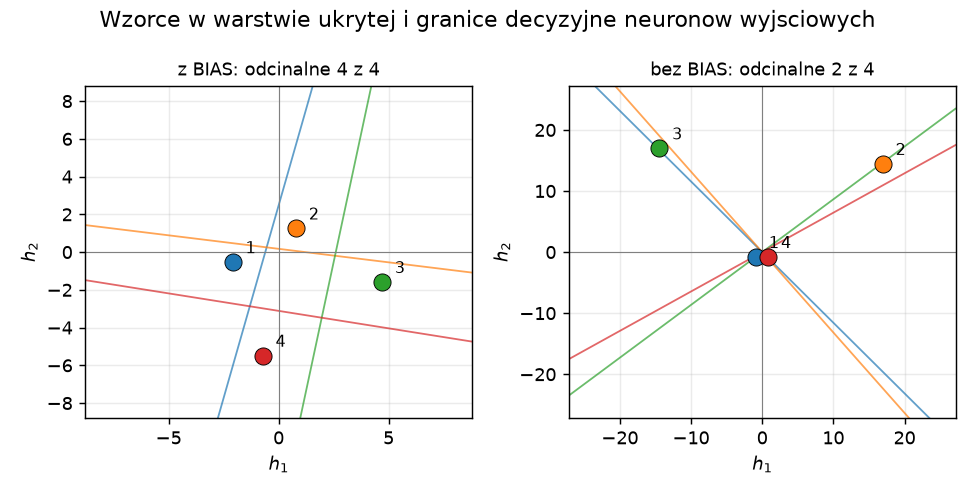
\includegraphics[width=\textwidth]{wyniki/geometria.png}
\caption{Wzorce w~warstwie ukrytej i~granice decyzyjne neuronów wyjściowych}
\label{fig:geometria}
\end{figure}

Wynik jest jednoznaczny i~taki sam dla obu wariantów: prostą dowolną da się
odciąć \textbf{4 z~4} punktów, a~prostą przechodzącą przez początek układu
tylko \textbf{2 z~4}. Nie zależy to od przebiegu treningu, bo jest własnością
czterech punktów na płaszczyźnie, a~nie konkretnych wag.

I~to zgadza się z~pomiarem: bez biasów poprawne są dokładnie dwa wzorce, bo
tylko dwa neurony wyjściowe są w~stanie wykonać swoje zadanie.

Na Rys.~\ref{fig:geometria} widać też, jak sieć bez biasów próbowała sobie
poradzić. Wszystkie cztery granice przechodzą przez punkt $(0,0)$, więc sieć
wypchnęła wzorce~2 i~3 bardzo daleko od środka, aż do wartości rzędu~17, gdzie
prosta przez początek układu potrafi je oddzielić. Wzorce~1 i~4 zostały
natomiast tuż przy początku, praktycznie jeden na drugim, i~tam żadna taka
prosta ich nie rozdzieli.

\section{Wnioski}

\paragraph{Czy perceptron dałoby się wytrenować bez wejść obciążających?}
Nie. Błąd zatrzymuje się na poziomie około $0{,}38$ wobec $0{,}00012$ przy
sieci z~biasami, czyli ponad 3300 razy wyżej, i~nie spada mimo wydłużania
treningu ani zmiany kroku uczącego. Dokładnie dwa z~czterech wzorców są
odtwarzane poprawnie; w~pozostałych dwóch sieć zapala właściwe wyjście, ale nie
potrafi wygasić fałszywego, które zostaje na poziomie $0{,}57$--$0{,}58$ zamiast
zera.

Jedno zastrzeżenie warto dodać. Gdyby za kryterium przyjąć samo wskazanie
neuronu o~najwyższym wyjściu, sieć bez biasów przeszłaby ten test: maksimum
wypada we właściwym miejscu we wszystkich czterech przypadkach. Trening
minimalizuje jednak funkcję~(\ref{eq:blad}), a~tej bez biasów zminimalizować się
nie da. W~sensie postawionego zadania trening jest więc nieskuteczny.

\paragraph{Jaka jest rola wejść obciążających?} Bias daje granicy decyzyjnej
\textbf{swobodę położenia}. Bez niego suma ważona wynosi $\mathbf{u}\cdot\mathbf{h}$, więc granica
$\mathbf{u}\cdot\mathbf{h} = 0$ zawsze przechodzi przez początek układu
współrzędnych. Z~biasem jest to pełna postać~(\ref{eq:granica}), czyli prosta
o~tym samym nachyleniu, ale przesunięta tam, gdzie trzeba.

Najprostsza analogia: $\mathbf{u}\cdot\mathbf{h}$ to prosta $y = ax$,
a~$\mathbf{u}\cdot\mathbf{h} + b$ to $y = ax + b$. Prostej przechodzącej przez
zero nie da się dopasować do danych, które wymagają wyrazu wolnego, i~nie pomoże
tu żadne dobieranie nachylenia.

W~tym zadaniu konsekwencja jest policzalna. Cztery punkty w~warstwie ukrytej
tworzą czworokąt wypukły, więc \emph{każdy} z~nich da się odciąć jakąś prostą.
Ale prostych przechodzących przez początek układu wystarcza tylko dla
\emph{dwóch} z~nich, bo dla pozostałych prosta musiałaby przejść „pomiędzy'',
a~przez zero tego nie zrobi. Stąd dwa poprawne wzorce zamiast czterech.

Drugi, bardziej obrazowy sposób: bez biasu zerowe wejście daje zerową sumę
ważoną, a~więc $f(0) = 0{,}5$ na każdym wyjściu. Sieć nie ma wtedy żadnego
sposobu, by mieć jakiekolwiek „domyślne nastawienie''. Bias jest właśnie tym
nastawieniem: mówi neuronowi, jak bardzo ma być skłonny się wzbudzić, zanim
jeszcze zobaczy jakiekolwiek wejście.

\section{Załączniki}

Konfiguracja sieci o~architekturze z~punktu 2.2 (plik \texttt{mlp.py}):

\begin{verbatim}
net = Network([4, 2, 4], bias=[False, use_bias],
              activations=[(linear, linear_derivative),
                           (sigmoid, sigmoid_derivative)])
\end{verbatim}

Aktywacja i~bias zadawane są osobno dla każdej warstwy: warstwa ukryta jest
liniowa i~bez biasu, wyjściowa sigmoidalna z~biasem.

\begin{thebibliography}{9}

\bibitem{wyklad}
K. Stokfiszewski.
\textit{Inteligentna Analiza Danych. Materiały do wykładu nr 2}.
Instytut Informatyki Politechniki Łódzkiej.

\bibitem{rumelhart}
D. E. Rumelhart, G. E. Hinton, R. J. Williams.
\textit{Learning representations by back-propagating errors}.
Nature 323, 1986.

\bibitem{osowski}
S. Osowski.
\textit{Sieci neuronowe do przetwarzania informacji}.
Oficyna Wydawnicza Politechniki Warszawskiej, Warszawa.

\end{thebibliography}

\end{document}
